\section{More on GANs and intro to Gradient Reversal Layers}

\subsection{A brief recap on Generative Adversarial Networks}

As we extensively discussed in Sec. \ref{sec:intro_GAN}, Generative Adversarial Networks (GANs) operate on a min-max game between two competing networks: a generator $G$ and a discriminator $D$. The generator tries to create realistic samples starting from random noise, while the discriminator acts as a binary classifier evaluating a mixture of real and fake samples, trying to distinguish between them. 

A useful analogy to understand this dynamic is the forger and the police officer. Initially, the forger (generator) produces very crude fake dollars, but as the police officer (discriminator) learns to identify the fakes, the forger is forced to become more sophisticated. Both networks improve in tandem. However, it is crucial to remember that the discriminator is merely a training tool: its sole purpose is to provide a loss function and gradients for the generator. Once the training is complete, the discriminator is discarded.

GANs have made incredible progress over the last decade, moving from generating blurry "dogs with three heads" in 2014 to photorealistic human faces and even playable video games from simple videos of people playing them, like PacMan or Grand Theft Auto. However, their training dynamics are notoriously unstable. 
As we already mentioned, they suffer from two major issues:
\begin{itemize}
    \item[-] \textit{Mode Collapse}: The generator might discover that producing one specific type of output (e.g., a perfect $\$50$ bill) fools the discriminator consistently. It will then collapse and only generate that single sample, ignoring the rest of the target distribution.
    \item[-] \textit{Vanishing Gradients}: If the discriminator becomes too perfect ($D(x_{\text{real}}) \to 1$ and $D(x_{\text{fake}}) \to 0$), the loss function plateaus. The generator receives no useful gradient updates and fundamentally does not know in which direction to adjust its weights to improve.
\end{itemize}

As we saw, the \textit{Wasserstein GAN (WGAN)} mathematically addresses this vanishing gradient issue by replacing the binary discriminator with a \textit{critic}. By computing the Earth Mover's distance between the real and fake distributions, the WGAN provides linear, non-vanishing gradients. However, this requires enforcing a Lipschitz continuous function, which is often non-trivial to implement in standard Deep Neural Networks.

\subsection{GANs today and the legacy of the Adversarial concept}

Today, Flow-based models and Diffusion models have largely superseded GANs in many pure generative tasks due to their superior stability and expressiveness. So, why should we still care about GANs?

The primary reason is \textit{speed}. Diffusion models require an iterative denoising process, which is computationally expensive during inference. GANs, once trained, generate data in a single forward pass. Because of this, they are still widely adopted in fields where inference speed is more critical than absolute accuracy, such as real-time video filters, medical physics (for fast dataset augmentation), and hybrid/distilled models.

More importantly, while the pure generative usage of GANs might be declining, the \textbf{"adversarial" concept itself is absolutely not dead}. It has evolved to solve a completely different class of problems: forcing a network to \textit{unlearn} specific features.

\subsection{Adversarial Unlearning and Gradient Reversal Layers}

Sometimes, your training sample contains information that you \textit{do not} want your network to use. We want to make the network more general and robust, ensuring it does not rely on nuisance information or dataset-specific biases. 

Simply removing a feature from your dataset is rarely enough, because the nuisance information is usually highly correlated with other features the network can still exploit. Let's look at three practical examples:
\begin{enumerate}
    \item \textit{Computer Vision}: You want to classify handwritten digits (MNIST) regardless of their color, but in your dataset, some numbers are always written in red and others in green. 
    \item \textit{High Energy Physics}: You want to build a jet tagger to recognize if a particle jet comes from a top quark, a Higgs boson, or a W boson. The invariant mass of the jet is highly discriminating, but you explicitly \textit{do not} want the network to use it. If the network learns the mass, applying a cut on the network's output will artificially "sculpt the background", creating fake mass peaks that ruin subsequent physics analyses.
    \item \textit{Medical Physics}: You have X-ray images from different hospital centers, each using different machines, resolutions, and contrast settings. You want to predict the biological age of patients, but you need the network to be "center-invariant" so it doesn't just learn to recognize which hospital the image came from.
\end{enumerate}

To solve this, we use \textbf{Adversarial Unlearning}. The idea is to add a dedicated \textit{Adversarial Head} to the early layers of our Deep Neural Network. While the main output head tries to solve the primary task (e.g., "which digit is it?"), the adversarial head tries to predict the nuisance variable (e.g., "what color is it?"), as shown in the following scheme.

\begin{center}
    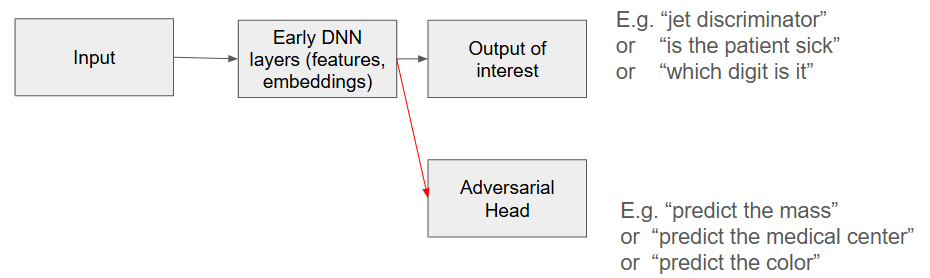
\includegraphics[width=0.8\textwidth]{figuresML_adv/lesson_ml_adv_6_pag_13.png}
\end{center}

We could train this architecture using a multi-step GAN-like loop: training the main head, then training the adversarial head while freezing the feature extractor, and finally updating the feature extractor to fool the adversarial head. However, there is a much more elegant and compact way to achieve this simultaneously: the \textbf{Gradient Reversal Layer (GRL)}. Take a look at this figure:

\begin{center}
    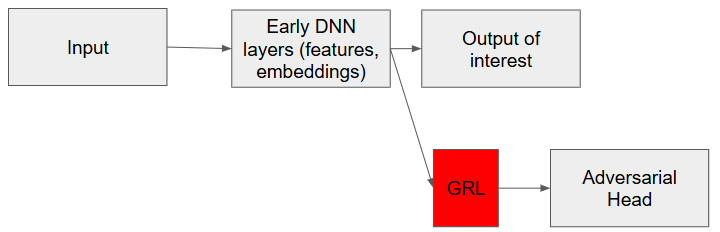
\includegraphics[width=0.6\textwidth]{figuresML_adv/lesson_ml_adv_6_pag_15.png}
\end{center}

The GRL is placed exactly between the feature extractor and the adversarial head. 
\begin{itemize}
    \item[-] During the \textbf{forward pass}, it acts as a simple identity function, doing absolutely nothing and letting the data flow to the adversarial head.
    \item[-] During \textbf{backpropagation}, it takes the gradient coming from the adversarial head and multiplies it by a negative scalar ($-\lambda$ or $-\alpha$).
\end{itemize}

This simple mathematical trick is extremely powerful. The adversarial head learns how to predict the nuisance variable as best as it can. But because the gradient is inverted by the GRL, the feature extractor updates its weights in the \textit{exact opposite direction}. The feature extractor is actively penalized if it retains any information useful to the adversarial head, forcing it to completely \textbf{unlearn} the nuisance variable and become domain-invariant. The total loss is simply the sum of the losses of the two heads.

\section{Practical implementation and hands-on examples}

Implementing adversarial training requires stepping outside the comfort zone of standard sequential wrappers. 

\textbf{GAN Training Loops in Keras} \\
If you use Keras, you must write your own custom training loop as shown in the example below. You manually iterate over the epochs, prepare real and fake samples, and use \texttt{train\_on\_batch()}. 
First, you train the discriminator on a mixture of real samples (label 1) and freshly generated fake samples (label 0). Then, to train the generator, you freeze the discriminator's weights, pass random noise through the combined generator-discriminator model, and set the target labels to 1. This forces the generator to update its weights to fool the frozen discriminator. 

\begin{Verbatim}[label=\makebox{\url{https://github.com/lucabaldini/cmepda/tree/master/slides/latex/snippets/gan_training.py}},commandchars=\\\{\}]
\PY{c+c1}{\PYZsh{} define the combined generator and discriminator model, for updating the generator}
\PY{k}{def}\PY{+w}{ }\PY{n+nf}{define\_gan}\PY{p}{(}\PY{n}{generator}\PY{p}{,} \PY{n}{discriminator}\PY{p}{)}\PY{p}{:}
    \PY{c+c1}{\PYZsh{} Step 1: freeze discriminator and compile the GAN}
    \PY{n}{discriminator}\PY{o}{.}\PY{n}{trainable} \PY{o}{=} \PY{k+kc}{False}
    \PY{n}{gan\_input} \PY{o}{=} \PY{n}{Input}\PY{p}{(}\PY{n}{shape}\PY{o}{=}\PY{p}{(}\PY{n}{generator}\PY{o}{.}\PY{n}{input\_shape}\PY{p}{[}\PY{l+m+mi}{1}\PY{p}{]}\PY{p}{,}\PY{p}{)}\PY{p}{)}
    \PY{n}{gan\_output} \PY{o}{=} \PY{n}{discriminator}\PY{p}{(}\PY{n}{generator}\PY{p}{(}\PY{n}{gan\_input}\PY{p}{)}\PY{p}{)}
    \PY{n}{gan\_model} \PY{o}{=} \PY{n}{Model}\PY{p}{(}\PY{n}{gan\_input}\PY{p}{,} \PY{n}{gan\_output}\PY{p}{)}
    
    \PY{c+c1}{\PYZsh{} slightly higher LR for generator so it can catch up with discriminator}
    \PY{n}{gan\_model}\PY{o}{.}\PY{n}{compile}\PY{p}{(}\PY{n}{loss}\PY{o}{=}\PY{l+s+s1}{\PYZsq{}}\PY{l+s+s1}{binary\_crossentropy}\PY{l+s+s1}{\PYZsq{}}\PY{p}{,} \PY{n}{optimizer}\PY{o}{=}\PY{n}{Adam}\PY{p}{(}\PY{l+m+mf}{3e\PYZhy{}4}\PY{p}{)}\PY{p}{)}
    
    \PY{c+c1}{\PYZsh{} Step 2: restore discriminator trainability for standalone training}
    \PY{n}{discriminator}\PY{o}{.}\PY{n}{trainable} \PY{o}{=} \PY{k+kc}{True}
    \PY{+w}{discriminator}\PY{o}{.}\PY{n}{compile}\PY{p}{(}\PY{n}{loss}\PY{o}{=}\PY{l+s+s1}{\PYZsq{}}\PY{l+s+s1}{binary\_crossentropy}\PY{l+s+s1}{\PYZsq{}}\PY{p}{,}\PY{+w}{ }
    \PY{+w}{                          }\PY{n}{optimizer}\PY{o}{=}\PY{n}{Adam}\PY{p}{(}\PY{l+m+mf}{1e\PYZhy{}4}\PY{p}{)}\PY{p}{,}\PY{+w}{ }\PY{n}{metrics}\PY{o}{=}\PY{p}{[}\PY{l+s+s1}{\PYZsq{}}\PY{l+s+s1}{accuracy}\PY{l+s+s1}{\PYZsq{}}\PY{p}{]}\PY{p}{)}
    
    \PY{k}{return} \PY{n}{gan\_model}

\PY{k}{def}\PY{+w}{ }\PY{n+nf}{train}\PY{p}{(}\PY{n}{g\_model}\PY{p}{,} \PY{n}{d\_model}\PY{p}{,} \PY{n}{gan\_model}\PY{p}{,} \PY{n}{latent\_dim}\PY{p}{,} \PY{n}{n\_epochs}\PY{p}{,} \PY{n}{n\_batch}\PY{p}{,} \PY{n}{n\_eval}\PY{p}{)}\PY{p}{:}
    \PY{n}{half\_batch} \PY{o}{=} \PY{n+nb}{int}\PY{p}{(}\PY{n}{n\_batch} \PY{o}{/} \PY{l+m+mi}{2}\PY{p}{)}
    
    \PY{k}{for} \PY{n}{i} \PY{o+ow}{in} \PY{n+nb}{range}\PY{p}{(}\PY{n}{n\_epochs}\PY{p}{)}\PY{p}{:}
        \PY{c+c1}{\PYZsh{} prepare real samples}
        \PY{n}{x\_real}\PY{p}{,} \PY{n}{y\_real} \PY{o}{=} \PY{n}{generate\_real\_samples}\PY{p}{(}\PY{n}{half\_batch}\PY{p}{)}
        
        \PY{c+c1}{\PYZsh{} prepare fake examples}
        \PY{n}{x\_fake}\PY{p}{,} \PY{n}{y\_fake} \PY{o}{=} \PY{n}{generate\_fake\_samples}\PY{p}{(}\PY{n}{g\_model}\PY{p}{,} \PY{n}{latent\_dim}\PY{p}{,} \PY{n}{half\_batch}\PY{p}{)}
        
        \PY{c+c1}{\PYZsh{} update discriminator}
        \PY{n}{d\_model}\PY{o}{.}\PY{n}{train\_on\_batch}\PY{p}{(}\PY{n}{x\_real}\PY{p}{,} \PY{n}{y\_real}\PY{p}{)}
        \PY{n}{d\_model}\PY{o}{.}\PY{n}{train\_on\_batch}\PY{p}{(}\PY{n}{x\_fake}\PY{p}{,} \PY{n}{y\_fake}\PY{p}{)}
        
        \PY{c+c1}{\PYZsh{} prepare points in latent space as input for the generator}
        \PY{n}{x\_gan} \PY{o}{=} \PY{n}{generate\_latent\_points}\PY{p}{(}\PY{n}{latent\_dim}\PY{p}{,} \PY{n}{n\_batch}\PY{p}{)}
        
        \PY{c+c1}{\PYZsh{} create inverted labels for the fake samples}
        \PY{n}{y\_gan} \PY{o}{=} \PY{n}{ones}\PY{p}{(}\PY{p}{(}\PY{n}{n\_batch}\PY{p}{,} \PY{l+m+mi}{1}\PY{p}{)}\PY{p}{)}
        
        \PY{c+c1}{\PYZsh{} update the generator via the discriminator\PYZsq{}s error}
        \PY{n}{gan\_model}\PY{o}{.}\PY{n}{train\_on\_batch}\PY{p}{(}\PY{n}{x\_gan}\PY{p}{,} \PY{n}{y\_gan}\PY{p}{)}
        
        \PY{c+c1}{\PYZsh{} evaluate the model every n\_eval epochs}
        \PY{k}{if} \PY{p}{(}\PY{n}{i}\PY{o}{+}\PY{l+m+mi}{1}\PY{p}{)} \PY{o}{\PYZpc{}} \PY{n}{n\_eval} \PY{o}{==} \PY{l+m+mi}{0}\PY{p}{:}
            \PY{n}{summarize\_performance}\PY{p}{(}\PY{n}{i}\PY{p}{,} \PY{n}{g\_model}\PY{p}{,} \PY{n}{d\_model}\PY{p}{,} \PY{n}{latent\_dim}\PY{p}{)}
\end{Verbatim}

\textit{Caveat}: Depending on the specific TensorFlow/Keras version, the behavior of the \texttt{trainable = False} flag can be highly buggy and non-obvious. Recompiling models dynamically inside a loop often leads to silent failures where layers remain frozen forever or unfreeze unexpectedly. This is one of the main reasons researchers often prefer PyTorch for custom adversarial architectures.

\textbf{Implementing the GRL in PyTorch} \\
In PyTorch, creating a GRL is beautifully simple thanks to the \texttt{torch.autograd.Function} class, which allows us to explicitly define custom forward and backward behaviors.

\begin{Verbatim}[label=\makebox{\url{https://github.com/lucabaldini/cmepda/tree/master/slides/latex/snippets/gradient_reversal.py}},commandchars=\\\{\}]
\PY{k}{class}\PY{+w}{ }\PY{n+nc}{GradientReversalLayer}\PY{p}{(}\PY{n}{torch}\PY{o}{.}\PY{n}{autograd}\PY{o}{.}\PY{n}{Function}\PY{p}{)}\PY{p}{:}
\PY{+w}{    }\PY{n+nd}{@staticmethod}
\PY{+w}{    }\PY{k}{def}\PY{+w}{ }\PY{n+nf}{forward}\PY{p}{(}\PY{n}{ctx}\PY{p}{,}\PY{+w}{ }\PY{n}{x}\PY{p}{,}\PY{+w}{ }\PY{n}{alpha}\PY{p}{)}\PY{p}{:}
\PY{+w}{        }\PY{c+c1}{\PYZsh{} Store alpha for the backward pass}
\PY{+w}{        }\PY{n}{ctx}\PY{o}{.}\PY{n}{alpha}\PY{+w}{ }\PY{o}{=}\PY{+w}{ }\PY{n}{alpha}
\PY{+w}{        }\PY{c+c1}{\PYZsh{} Forward pass: act as an identity function}
\PY{+w}{        }\PY{k}{return}\PY{+w}{ }\PY{n}{x}\PY{o}{.}\PY{n}{view\_as}\PY{p}{(}\PY{n}{x}\PY{p}{)}

\PY{+w}{    }\PY{n+nd}{@staticmethod}
\PY{+w}{    }\PY{k}{def}\PY{+w}{ }\PY{n+nf}{backward}\PY{p}{(}\PY{n}{ctx}\PY{p}{,}\PY{+w}{ }\PY{n}{grad\_output}\PY{p}{)}\PY{p}{:}
\PY{+w}{        }\PY{c+c1}{\PYZsh{} Backward pass: multiply the gradient by \PYZhy{}alpha}
\PY{+w}{        }\PY{n}{output}\PY{+w}{ }\PY{o}{=}\PY{+w}{ }\PY{n}{grad\_output}\PY{o}{.}\PY{n}{neg}\PY{p}{(}\PY{p}{)}\PY{+w}{ }\PY{o}{*}\PY{+w}{ }\PY{n}{ctx}\PY{o}{.}\PY{n}{alpha}
\PY{+w}{        }\PY{k}{return}\PY{+w}{ }\PY{n}{output}\PY{p}{,}\PY{+w}{ }\PY{k+kc}{None}
\end{Verbatim}

\subsubsection{Hands-on examples on GANs and GRLs}
To solidify these concepts, we will jump into two practical exercises:
\begin{itemize}
    \item[-] \textit{GAN Exercise}: We will create a target 2D distribution (e.g., points arranged in a circle or a ring) and build a GAN from scratch to reproduce it starting from random noise. You can access the Notebook at the following link: \url{https://colab.research.google.com/drive/1-8NUePIpozh0DyMD3gk0DKcuLukhHcCR?usp=sharing}.
    \item[-] \textit{GRL Exercise}: We will tackle a dataset containing two distinct features: a "Class" we want to predict, and a "Domain" we want to ignore (acting as a distractor). We will demonstrate how standard networks fail by implicitly learning the domain, and how introducing a GRL makes the transformed feature space fully domain invariant, making the network robust even if the test dataset has a completely different domain mix. Here is the link to the Notebook: \url{https://colab.research.google.com/drive/1la6rC_umcygR5g_mbnL15ZGd3aNkpNsP?usp=sharing}.
\end{itemize}

%\includepdf[pages=-, pagecommand={\thispagestyle{plain}}]{lezioni/e_ML_adv_6Ahands_on.pdf}

% ML_11a nel mio colab

%\includepdf[pages=-, pagecommand={\thispagestyle{plain}}]{lezioni/e_ML_adv_6Bhands_on.pdf}

% ML_11b nel mio colab